\pagestyle{fancy}
\renewcommand{\theUnit}{5}
\ifthenelse{\isundefined{\UnitPageNumbers}}{}{\setcounter{page}{1}}
\rhead{Chapter \theUnit: Bootstrap Distributions}
\lhead{Math 3382: Statistical Theory}
%\lhead{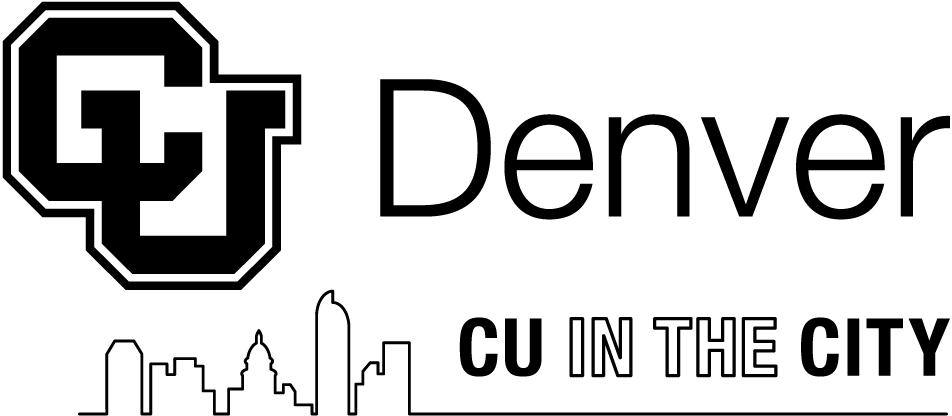
\includegraphics[width=1.25cm]{CUDenver-Logo.png}}
\rfoot{\mypage}
\cfoot{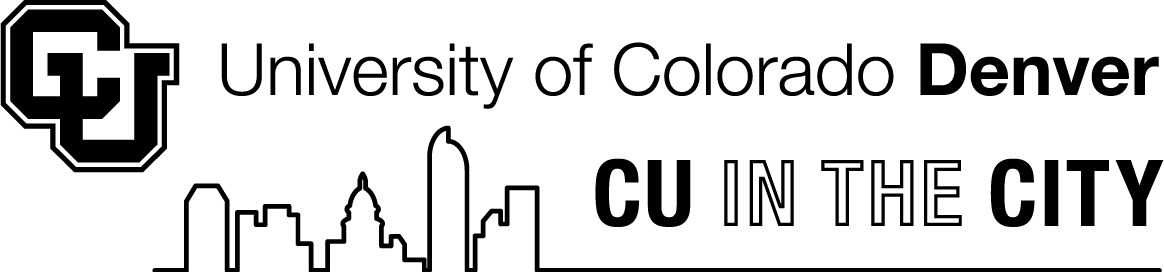
\includegraphics[width=2.25cm]{CUDenver-Logo-coverpage.png}}
\lfoot{Adam Spiegler}
\fancypagestyle{firstfooter}{\footskip = 50pt}
\renewcommand{\footrulewidth}{.4pt}
%%%%%%%%%%%%%%%%%%%%%%%%%%%
\vspace*{-20pt} \thispagestyle{firstfooter}


%\begin{tasks}[counter-format = {(tsk[a])},label-offset = {0.8em},label-format = {\color{black}\bfseries}](2)


\pagebegin{Section 5.5: Bootstrap Distributions with Other Statistics}

\bbox
Some statistics, such as means and proportions, we can prove a theory such as the Central Limit Theorem that allows us to theoretically model sampling distributions for those statistics.

\bi
\ii Not all statistics have a Central Limit Theorem.
\ii The bootstrap procedure may be used with a wide variety of other statistics, such as medians, trimmed means, covariance, and ratios.
\ii \textbf{\colorb{We can construct a bootstrap distribution to estimate the sampling distribution for any statistic, even if there is no Central Limit Theorem.}}
\ei
\ebox

\bb
\ii Verizon is the incumbent local exchange carrier (ILEC) for a large part of the Eastern US. When there is an emergency Verizon is responsible for making repairs for the customers of other telephone companies in the region known as competing local exchange carriers (CLEC's). Verizon is subject to fines if the repair times for CLEC customers are substantially worse than the times for Verizon customers. The dataset \textit{Verizon} contains a sample of repair times (\textit{Time}) for 1664 ILEC and 23 CLEC customers (\textit{Group}). Rather than estimate the difference in mean times, suppose we look at the ratio of the means, what is the ratio of the ILEC mean repair time over the CLEC mean repair time?  \textbf{Construct a 95\% bootstrap confidence interval for the ratio of the two means.} \label{verizon-ratio}\bigskip

Time.ILEC $<-$ subset( Verizon, select = \_\_\_\_\_\_\_\_\_\_\_\_\_\_\_\_  , Group == ``\_\_\_\_\_\_\_\_\_\_\_\_\_'', drop = T)\\
Time.CLEC $<-$ subset( Verizon, select = \_\_\_\_\_\_\_\_\_\_\_\_\_\_\_\_  , Group == ``\_\_\_\_\_\_\_\_\_\_\_\_\_ '', drop = T)\\ 
\\
N $<- 10^5$\\
boot.ratio.mean $<-$ numeric(N)\\
for (i in 1:N)\\
$\left\{ \right.$\\
\indent \ \ \ \ \ \ ILEC.sample $<-$ sample(\_\_\_\_\_\_\_\_\_\_ , \_\_\_\_\_\_\_\_\_\_ , replace = \_\_\_\_\_\_\_\_\_\_ )\\
\indent \ \ \ \ \ \ CLEC.sample $<-$ sample(\_\_\_\_\_\_\_\_\_\_ , \_\_\_\_\_\_\_\_\_\_ , replace = \_\_\_\_\_\_\_\_\_\_)\\
\indent \ \ \ \ \ \ boot.ratio.mean[i] $<-$ \_\_\_\_\_\_\_\_\_\_\_\_\_\_\_\_\_\_\_\_\_\_\_\_\_\_\_\_\_\_  \\
$\left. \right\}$\\
\\
lower $<-$ quantile( \_\_\_\_\_\_\_\_\_\_\_\_\_\_\_\_\_\_\_\_\_\_\_\_\_\_\_\_\_  ,  \_\_\_\_\_\_\_\_\_\_\_\_\_) \\
upper $<-$ quantile( \_\_\_\_\_\_\_\_\_\_\_\_\_\_\_\_\_\_\_\_\_\_\_\_\_\_\_\_\_  ,  \_\_\_\_\_\_\_\_\_\_\_\_\_)\\
\\
original.ratio $<-$ \_\_\_\_\_\_\_\_\_\_\_\_\_\_\_\_\_\_\_\_\_\_\_\_\_\_\_\_  \#ratio of original sample means. \\
mean.boot $<-$  \_\_\_\_\_\_\_\_\_\_\_\_\_\_\_\_\_\_\_\_\_\_\_\_  \#mean of the bootstrap dist for ratio of sample means\\
\\
hist( \_\_\_\_\_\_\_\_\_\_\_\_\_\_\_\_\_\_\_\_\_\_\_\_\_\_\_\_\_  , main = ``Bootstrap dist of the ratio of means'')\\
abvline(v = mean.boot , col = ``red'', lty = 2) \\
abvline(v = original.ratio , col = ``blue'', lty = 2) \\
\\
qqnorm( \_\_\_\_\_\_\_\_\_\_\_\_\_\_\_\_\_\_\_\_\_\_\_\_\_\_\_\_\_ )\\
qqline( \_\_\_\_\_\_\_\_\_\_\_\_\_\_\_\_\_\_\_\_\_\_\_\_\_\_\_\_\_ )\\
\ee


\clearpage

\begin{multicols}{2}

\begin{center}
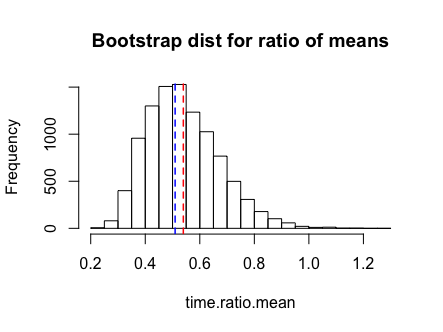
\includegraphics[width=0.4\tw]{13/fig-verizon-ratio.png}
\end{center}

\[ \mbox{95\% Bootstrap CI} = 0.328 \mbox{ to } 0.837.\]
\[ \mbox{Ratio from Original Sample} = \frac{\bar{x}_{\rm{ILEC}}}{\bar{x}_{\rm{CLEC}}} = \colorb{0.5095}.\]
\[ \mbox{Bootstrap center}  = \colorr{0.5396}.\]

\columnbreak

\begin{center}
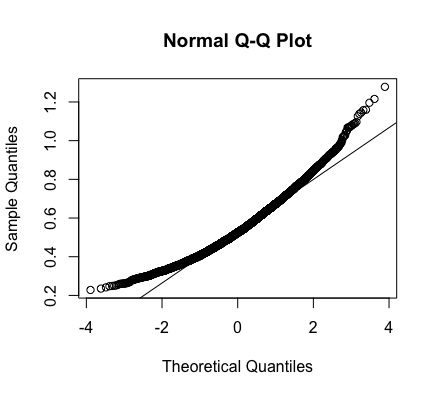
\includegraphics[width=0.4\tw]{13/fig-verizon-qq.png}
\end{center}

\end{multicols}


\pagebegin{Section 5.6: Bias}

\bbox
\bi
\ii Let $\theta$ denote a parameter. We denote an \textbf{\colorb{estimator}} for the parameter with a hat, \textbf{\colorb{$\widehat{\theta}$}}.
\ii An estimator $\hat{\theta}$ is \textbf{\colorb{biased}} if on average it tends to be too high or too low relative to the true value of $\theta$. The bias of an estimator is
\[ \mbox{Bias}\lbrack \hat{\theta} \rbrack = \Exp \lbrack \hat{\theta} \rbrack - \theta.\]
\ii The bootstrap estimate of bias is
\[ \mbox{Bias}_{\rm{boot}} \lbrack \hat{\theta}^{\ast} \rbrack =  \Exp \lbrack \hat{\theta}^{\ast} \rbrack - \hat{\theta}.\]
\bi
\ii[$\circ$]  $\Exp \lbrack \hat{\theta}^{\ast} \rbrack$ denotes the center of the bootstrap distribution.
\ii[$\circ$]  $\hat{\theta}$ denotes the sample statistic.
\ei
\ii An estimator is \textbf{\colorb{unbiased}} if the bias is zero.
\ei
\ebox


\bb[resume]
\ii  Using the output from the previous bootstrap distribution, calculate the bootstrap estimate of bias in the previous Verizon example \ref{verizon-ratio}. \bigskip

\begin{center}
\begin{tabular}{|l|l|l|}
$\mbox{E} \lbrack \hat{\theta}^{\ast} \rbrack$ \ \ \ \ \ \ \ \ \ \ & $\hat{\theta}$ \ \ \ \ \ \ \ \ \ \ \ \ \ \ \ & $\mbox{Bias}_{\rm boot} \lbrack \hat{\theta}^{\ast} \rbrack$ \ \ \ \ \ \ \ \ \\
\hline
 & & \\
 \end{tabular}
 \end{center}

%\ii Consider a sample $X_1, X_2, \ldots X_n$ randomly selected from population $X$  and $Y_1, Y_2, \ldots Y_m$ randomly selected from population $Y$. Show that the difference in sample means, $\bar{X} - \bar{Y}$, is an unbiased estimator for the difference in population means, $\mu_X - \mu_Y$. \vfill
\ee

\clearpage

\bbox
\bi
\ii We can measure how extreme is the bias of an estimator using the ratio
\[ \frac{\mbox{Bias}}{\mbox{SE}} \approx  \frac{\mbox{Bootstrap Bias}}{\mbox{Bootstrap SE}}.\]
\ii \colorb{\textit{Rule of Thumb:} \textbf{If the ratio bias/SE exceeds $\pm 0.02$, then the bias is large enough to have a substantial effect on the accuracy of the estimate.}}
\ei
\ebox

\bb[resume]
\ii In the arsenic example \ref{q:arsenic} we used a bootstrap distribution to estimate the mean arsenic level (in ppb)
present in groundwater in Bangladesh. The mean of the original sample is $\bar{x} = 125.320$. The mean
of a bootstrap distribution is $125.229$. A bootstrap standard error
is $17.9$. Which bias is more extreme, the bias in the arsenic or Verizon example?
\ee

\vfill

\pagebegin{Sections 5.7-5.9: Implementation and Accuracy}

\bb[resume]
\ii If we had a sample $\left\{ 10,  20 , 18 \right\}$, how many possible bootstrap samples are there? \vfill

\ee

In the Verizon example, there are at most $1664^{1664} \cdot 23^{23}$ different bootstrap samples, If there are
duplicate values in the sample(s), then it gets even more tricky to avoid repeats.

\bbox
\bi
\ii We have not been ensuring we generate all possible bootstrap samples while avoiding repeats.
\ii We have used \textbf{\colorb{Monte Carlo sampling}} which gives an estimate of the theoretical bootstrap distribution.
\ii The larger the number of bootstrap samples, the better the estimate. As a rule, $N=10^4$ bootstrap samples or more is sufficient.
\ei
\ebox
